\documentclass[aspectratio=169]{beamer}
\usetheme[logo]{hypro} % the template, use option "wwu" instead of "logo" to set the footer
\usepackage[useregional]{datetime2} % nice date typesetting
\usepackage{csquotes} % to quote stuff via \enquote{stuff}
\usepackage{xspace} % automated spacing after macros
\usepackage[normalem]{ulem} % allows to strikethrough text via \sout{text}
\usepackage{siunitx} % for nice units
\usetikzlibrary{calc,decorations.markings,arrows.meta,automata,backgrounds,positioning,intersections,shapes,decorations.pathreplacing,positioning,patterns}

\title{Optimizing reachability probabilities for a restricted class of Stochastic Hybrid Automata via Flowpipe-Construction}
\author[Stefan Schupp]{Carina Pilch, \textbf{Stefan Schupp}, Anne Remke}
\date{\DTMdisplaydate{2021}{7}{7}{-1}}

%################ Commands
\newcommand{\cb}[1]{\textcolor{blue100}{#1}\xspace}



\begin{document}

\begin{frame}[plain]
	\begin{centering}
		\vspace*{0.5cm}
		\begin{beamercolorbox}[sep=8pt,center]{title}
			\usebeamerfont{title}\inserttitle\par%
			\ifx\insertsubtitle\@empty%
			\else%
			\vskip0.25em%
			{\usebeamerfont{subtitle}\usebeamercolor[fg]{subtitle}\insertsubtitle\par}%
			\fi%
		\end{beamercolorbox}%
		\vskip1em\par
		\begin{beamercolorbox}[sep=8pt,center]{author}
			\usebeamerfont{author}\insertauthor
		\end{beamercolorbox}
		\begin{beamercolorbox}[sep=8pt,center]{institute}
			
			
\includegraphics[height=1cm]{pics/TU_logo.png}\hspace{.5cm}
\includegraphics[height=1cm]{pics/wwu.png}
			
			\usebeamerfont{institute}\insertinstitute
		\end{beamercolorbox}
		\begin{beamercolorbox}[sep=8pt,center]{date}
			\usebeamerfont{date}\insertdate
		\end{beamercolorbox}%\vskip0.5em
		\vfill
		\if@dfg
		\vspace*{1cm}
		\tiny
		This work is part of the project HyPro
		\if@unravel
		and the Research Training Group 2236 UnRAVeL
		\fi
		\\
		\href{http://ths.rwth-aachen.de/research/hypro/}{\includegraphics[width=.15\paperwidth]{pics/hypro_logo.png}}
		\if@unravel
		\qquad
		\href{https://moves.rwth-aachen.de/research/projects/unravel/}{\includegraphics[width=.15\paperwidth]{pics/rwth_unravel_bild_rgb.png}}\\
		\else
		\\
		\fi
		which
		\if@unravel
		are
		\else
		is
		\fi
		funded by the German Research Council (DFG).
		\else
		\if@unravel
		\tiny
		This work is part of the  Research Training Group 2236 UnRAVeL\\
		\href{https://moves.rwth-aachen.de/research/projects/unravel/}{\includegraphics[width=.15\paperwidth]{pics/rwth_unravel_bild_rgb.png}}\\
		which is funded by the German Research Council (DFG).
		\else
		\vspace*{1.6cm}
		\fi
		\fi

	\end{centering}
	% adjust page count
	\addtocounter{framenumber}{-1}
	%\vfill
\end{frame}

%########################################################

\begin{frame}{The problem in a nutshell}
  \enquote{\alert<2>{Optimizing \alert<1>{reachability probabilities}} for a \alert<5>{restricted class of \alert<4>{Stochastic \alert<3>{Hybrid Automata}}} via \alert<6>{Flowpipe-Construction}}

  \bigskip

  \only<3>{Hybrid automata: a model for \emph{hybrid systems}

  \medskip

  \cb{\faArrowRight} mixed discrete-continuous behavior
  }%
  \only<4>{Stochastic hybrid automata: a model for \emph{stochastic} hybrid systems

  \medskip

  \cb{\faArrowRight} add stochasticity
  \begin{itemize}
    \item continuous behavior: e.g., stochastic differential equations
    \item discrete behavior: e.g., stochastic jumps
  \end{itemize}
  }%
  \only<5>{Stochastic hybrid automata: a model for \emph{stochastic} hybrid systems

  \medskip

  \cb{Here:}
  \begin{itemize}
    \item \sout{continuous behavior: e.g., stochastic differential equations}
    \item discrete behavior: \cb{urgent} jumps and \cb{stochastic} jumps
    \item \cb{singular automata}
    \begin{itemize}
      \item constant derivatives
      \item predicates compare variables to constants (\enquote{axis-aligned})
    \end{itemize}
  \end{itemize}

  \bigskip

  \cb{Stochasticity:} continuous probability distributions
  }%
  \only<1>{\cb{Question:} What is the probability, given a set of initial states of reaching a set of \emph{goal states}?

  \bigskip

  Example: Stochastic jumps
  \begin{itemize}
    \item Are taken \enquote{randomly}
    \item The probability of taking this jump is given by a continuous densitiy function

    \cb{Intuition:} The probability of taking this jump increases with passage of time
  \end{itemize}

  %\medskip
  %Non-stochastic jumps
  %\begin{itemize}
  %  \item Guards only on continuous variables
  %  \item Potentially introduce non-determinism
  %\end{itemize}


  }%
  \only<2>{\cb{Question:} What is the \alert{maximal/minimal} probability, given a set of initial states of reaching a set of \emph{goal states}?

  \bigskip

  \cb{Observation:} There may be several ways (here: discrete non-determism) to reach a goal state


  \medskip
  Dealing with discrete choices
  \begin{itemize}
    \item Currently: Over-approximate (e.g., via state space discretization) probabilities for discrete non-determinism.
    \item Here: Exact probabilities (up to numerical integration)
  \end{itemize}

  }%
  \only<6>{\cb{Idea:} represent sets of reachable states by geometric shapes
  \begin{itemize}
    \item Usually over-approximative, here: \cb{exact}
    \item Different types of representations, here: \cb{convex polyhedra}
  \end{itemize}

  \vspace*{.7cm}

  \begin{minipage}{.5\linewidth}
    \scriptsize Time elapse

    \centering
    \begin{tikzpicture} [
    stateSetUnbounded/.style={fill=blue100, fill opacity=0.2}
    ,stateSetBounded/.style={stateSetUnbounded,draw,thick}
    , vector/.style={draw,thick,>=latex,->}
    , >=latex
    , every node/.style={font=\scriptsize}
    , scale=0.7
]
    % coordinate system
    %\draw[help lines] (0,0) grid ($(7,4) + (-\pgflinewidth, -\pgflinewidth)$);
    \draw[thick,->] (0,0) -- node[pos=1,below]{$x_0$}(7,0);
    \draw[thick,->] (0,0) -- node[pos=1,left]{$x_1$}(0,4);

    \begin{scope}
    \clip (0,0) rectangle (7,4);

    % invariant
    \path[stateSetUnbounded, fill opacity=0.1] (0,0) rectangle (5,4);
    \draw[thick] (5,0) -- (5,4);
    %\path[vector] (5,2.5) -- (5.5,2.5);

    % time elapse successors
    \path[stateSetUnbounded] (1,1) -- (2,1) -- (10,3) -- (10,4.25) -- (1,2) -- cycle;
    % initial set
    \path[stateSetBounded] (1,1) rectangle (2,2);

    % rays
    \path[vector] (2,1) -- (4,1.5);
    \path[vector] (2,2) -- (4,2.5);
    \path[vector] (1,2) -- (3,2.5);
    \path[vector] (1,1) -- (3,1.5);

    % time elapse intersected with the invariant (just borders)
    \draw[thick] (1,1) -- (2,1) -- (5,1.75) -- (5,3) -- (1,2) -- cycle;

    \end{scope}

    % labels
    %\node[right, anchor=south east ,text width=1.65cm] at(5,0) %{\scriptsize\begin{align*}
    %    \mathit{Act}(l)_0 &= 2\\
    %    \mathit{Act}(l)_1 &= 0.5
    %\end{align*}};
    \node[anchor=east] at(5,3.75) {$\mathit{Inv}(l)$};

    \node[] at(1.5,1.5) {$V$};
    \node[] at(6,2.5) {$V^+$};%\downarrow_{\mathit{Var}}$};
    \node[anchor=west] at(2.3,1.9) %{$(V^+\downarrow_{\mathit{Var}})\cap\mathit{Inv}(l)$};
    {$V^+\cap\mathit{Inv}(l)$};
    %\node[below] at(4,1.5) {$\begin{pmatrix}
    %2 \\
    %0.5
    %\end{pmatrix}$};
    %\node[below] at(6,2.5) {$\begin{pmatrix}
    %1 \\
    %0
    %\end{pmatrix}$};

\end{tikzpicture}

  \end{minipage}%
  \begin{minipage}{.5\linewidth}
    \scriptsize Jump successors (reset $x_0$)

    \centering
    \begin{tikzpicture} [
    stateSetUnbounded/.style={fill=blue100, fill opacity=0.2}
    ,stateSetBounded/.style={stateSetUnbounded,draw,thick}
    , vector/.style={draw,thick,>=latex,->}
    , >=latex
    , every node/.style={font=\scriptsize}
    , scale=0.7
]
    % coordinate system
    %\draw[help lines] (0,0) grid ($(7,4) + (-\pgflinewidth, -\pgflinewidth)$);
    \draw[thick,->] (0,0) -- node[pos=1,below]{$x_0$}(7,0);
    \draw[thick,->] (0,0) -- node[pos=1,left]{$x_1$}(0,4);

    \begin{scope}
    \clip (0,0) rectangle (7,4);

    % time elapse successors
    \path[stateSetBounded, fill opacity=0.2, thin] (1,-1) -- (3.5,-1) -- (5.5,1) -- (5.5,3.5) -- cycle;

    % guard
    \path[stateSetBounded, xshift=4cm, orange100] (1.5,-1) rectangle (6.5,5);
    \draw[orange100, line width=1mm] (5.5,1) -- (5.5,3.5);

    % projected set
    \path[stateSetBounded, dashed, fill=none] (-1,1) rectangle (10,3.5);
    % post_0
    \draw[green100, line width=1mm, opacity=0.2] (1,-1) -- (1,10);

    % reset set
    \draw[green100, line width=1mm] (1,1) -- (1,3.5);

    \end{scope}

    % labels
    \node[] at(3.75,0.5) {$V$};
    \node[right, orange100] at(5.5,2.25) {$V^{\mathit{pre}}$};
    \node[above, orange100] at(6.25,0) {$\mathit{pre}$};
    %\node[] at(3,2.25) (projection) {$V^{proj}$};
    %\draw[line width=1mm] (0,1) -- (0,3.5);
    \node[right, green100] at(1,2.25) {$V^{\mathit{post}}$};
    \node[above right, green100] at(1,0) {$\mathit{post}_0$};
    \node[anchor=east] at(5.5,3.75){$\mathit{Inv}(l)$};

\end{tikzpicture}

  \end{minipage}%
  }%
\end{frame}

%########################################################

\begin{frame}{The approach}

  \begin{enumerate}
    \item Compute forwards reachability (flowpipe construction)
    \begin{itemize}
      \item Keep track of non-determistic choices $\rightarrow$ \emph{reach tree}
      \item Stochasticity via \emph{random clocks} (one per enabled jump)
    \end{itemize}
    \item Collect paths in the reach tree which lead to a goal state
    \item Compute \emph{optimal} probability of those paths with respect to different \emph{schedulers}
  \end{enumerate}

  \bigskip

  \centering
  \begin{reminder}{\footnotesize Info: Scheduler}{9cm}
    \footnotesize
    Intuition: a scheduler resolves discrete non-determinism

    Different types, relevant here:
    \begin{itemize}
      \item History-dependent (knows past decisions),
      \item Prophetic (knows all expiration times) vs. non-prophetic (does not know expiration times)
    \end{itemize}
  \end{reminder}
\end{frame}

%########################################################

\begin{frame}{Flowpipe construction \& reach tree}

  \begin{minipage}{.7\linewidth}
    \begin{itemize}
      \item Constant derivatives result in conic sets for time-successors
      \item Random variables as clocks
      \item Two types of jumps
      \begin{itemize}
        \item Urgent, guarded jumps:
          \begin{itemize}
            \item Leave location once an urgent discrete jump is enabled
            \item Jump time is deterministic
          \end{itemize}
          \item Stochastic jumps:
          \begin{itemize}
            \item Unguarded (always enabled, no restriction on stochasticity)
            \item Clocks track \enquote{enabling time}
            \item Clock disabled (globally) after taking stoch. jump
          \end{itemize}
      \end{itemize}
    \end{itemize}
  \end{minipage}%
  \begin{minipage}{.3\linewidth}
      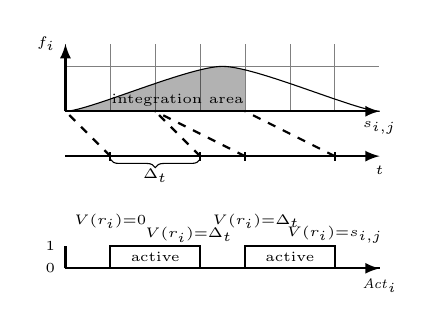
\begin{tikzpicture}
[
scale=.57
, >=latex
, every node/.style={font=\tiny}
]

\draw[help lines] (0,0) grid ($(7,1.5) + (-\pgflinewidth,-\pgflinewidth)$);
\draw[thick,->] (0,0) -- node[below,pos=1]{$s_{i,j}$}(7,0);
\draw[thick,->] (0,0) -- node[left,pos=1]{$f_{i}$} (0,1.5);

% CDF
\draw[name path=function] (0,0) .. controls (0.5,0) and (2.75,1) .. (3.5,1) .. controls (4.25,1) and (6.5,0) .. (7,0);

% CDF intersections
\path[name path=tmax] (4.5,-1) -- (4.5,1.5);
\path[name path=act] (1,-1) -- (1,1.5);
\path[name path=dis] (3,-1) -- (3,1.5);
\path[name path=react] (4,-1) -- (4,1.5);
\path [name intersections={of=function and tmax,by=tmaxf}];
\path [name intersections={of=function and act,by=actf}];
\path [name intersections={of=function and dis,by=disf}];
\path [name intersections={of=function and react,by=reactf}];

% step function: Act_i
\begin{scope}[yshift=-3.5cm]
\draw[thick] (0,0) -- (1,0) -- (1,0.5) -- (3,0.5) -- (3,0) -- (4,0) -- (4,0.5) -- (6,0.5) -- (6,0) -- (7,0);
\draw[thick,->] (0,0) -- node[below,pos=1]{$\mathit{Act}_i$}(7,0);
\draw[thick] (0,0) -- node[pos=0,left]{$0$} node[pos=1,left]{$1$} (0,0.5);
\end{scope}

% global time
\begin{scope}[yshift=-1cm]
\draw[thick,->] (0,0) -- node[below,pos=1]{$t$}(7,0);
\draw[thick] (1,-.1) -- (1,.1);
\draw[thick] (3,-.1) -- (3,.1);
\draw[thick] (4,-.1) -- (4,.1);
\draw[thick] (6,-.1) -- (6,.1);
\end{scope}

% mark valuations
\begin{scope}
\clip (0,-.5) rectangle (2,1.5);
\fill[fill=black, fill opacity=0.3] (0,0) .. controls (0.5,0) and (2.75,1) .. (3.5,1) .. controls (4.25,1) and (6.5,0) .. (7,0) -- cycle;
%\fill[fill=black, fill opacity=0.15] (0,0) rectangle (3,-.5);
\end{scope}
\draw[dashed, thick](1,-1) -- (0,0);
\draw[dashed, thick](3,-1) -- (2,0);
\begin{scope}
\clip (2,0) rectangle (4,1.5);
\fill[fill=black, fill opacity=0.3] (0,0) .. controls (0.5,0) and (2.75,1) .. (3.5,1) .. controls (4.25,1) and (6.5,0) .. (7,0) -- (7,-3) -- (0,-3) -- cycle;
\end{scope}
%\fill[fill=black, fill opacity=0.15] (4,-0.5) .. controls (4,-.25) and (3,-.25) .. (3,0) -- (5,0) .. controls (5,-.25) and (6,-.25) .. (6,-0.5) -- cycle;
\draw[dashed, thick](4,-1) -- (2,0);
\draw[dashed, thick](6,-1) -- (4,0);

% labels
\node[] at (1,-2.45){$\scriptscriptstyle V(r_i) = 0$};
\node[] at (2.75,-2.75){$\scriptscriptstyle V(r_i) = \Delta_t$};
\node[] at (4.25,-2.45){$\scriptscriptstyle V(r_i) = \Delta_t$};
\node[] at (2,-3.25){active};
\node[] at (5,-3.25){active};
\node[] at (6,-2.75){$\scriptscriptstyle V(r_i) = s_{i,j}$};
\node[] at (2.5,.25){integration area};
\begin{scope}[yshift=.5cm]
  \draw [decorate,decoration={brace,amplitude=3pt},xshift=0pt,yshift=-2pt]
  (3,-1.5) -- (1,-1.5) node [anchor=north,midway]
  {\tiny $\Delta_t$};
\end{scope}


%intersection
%\path[name path=tmax] (4.5,-1) -- (4.5,1.5);
%\path [name intersections={of=function and tmax,by=E}];

%\draw[thick] (1,-.25) -- node[fill=white,below, pos=0]{$\val(c_i) = 0$} (1,-0.75);
%\draw[thick] (4.5,-1.25) -- node[fill=white,below, pos=0]{$\val(c_i) = s_i$} (E);
%\node[fill=white] at(1,-0.5) {activation};
%\node[fill=white] at(4.5,-0.5) {expiration};

\end{tikzpicture}

  \end{minipage}

  \begin{result}{In a nutshell}{\linewidth}
    Non-determinism only over non-stochastic jumps
    \begin{itemize}
      \item Time point is fixed (urgent)
      \item In case several jumps are enabled: non-deterministic choice ($\rightarrow$ reach tree)
    \end{itemize}
  \end{result}

\end{frame}

%########################################################

\begin{frame}{Relevant paths}
After the analysis of the purely hybrid model (flowpipe construction) a \emph{reach tree} collects all state sets and discrete branchings
\begin{itemize}
  \item Nodes: represent passage of time, store flowpipe segments
  \item Parent-child relation: represents a discrete jump (stochastic or non-stochastic)
\end{itemize}

\bigskip

\cb{Approach}
\begin{itemize}
  \item Determine sets of reachable states that satisfy the goal-condition (intersection)
  \item A path in the reach tree to such a state set represents a sequence of discrete jumps (stochastic and non-stochastic)
  \begin{itemize}
    \item Stochastic jumps: The valuation of the random clock for this jump determines the probability to reach a goal state
    \item Non-stochastic jumps: Non-determinism needs to be resolved by a scheduler
  \end{itemize}
\end{itemize}





\end{frame}

%########################################################

\begin{frame}{Projection on random clocks}

  After the analysis, the reach tree contains sets of reachable states which contain
  \begin{itemize}
    \item Reachable valuations for continuous variables
    \item Reachable valuations for random clocks
  \end{itemize}

  \medskip

  From now on: Only require valuations of random clocks (projection)
  \begin{itemize}
    \item Used for integration
    \item Non-expired clocks require special handling (\enquote{lifting})
  \end{itemize}

  \bigskip

  \centering
  \begin{tikzpicture}
[
    stateSetUnbounded/.style={fill=blue100, fill opacity=0.2}
    ,stateSetBounded/.style={stateSetUnbounded,draw,thick}
    ,vector/.style={draw,thick,>=latex,->}
    ,>=latex
    , every node/.style={font=\small}
]

%\draw[help lines] (0.8,0) grid ($(7,2)+(-\pgflinewidth,-\pgflinewidth)$);
\draw[thick,->] (0.8,0) -- node[pos=1,below, xshift=-.3cm]{\scriptsize$s_{0,j}$}(5.75,0);
\draw[thick,->] (0.8,0) -- node[pos=1,right]{\scriptsize$x_0$}(0.8,2);


% state set
\path[stateSetBounded] (1,0) -- (3,0) -- (4,1.5) -- (2,1.5) -- cycle;
% state set reduced to goal states
\path[stateSetBounded] (1.66666,1) -- (3.66666,1) -- (4,1.5) -- (2,1.5) -- cycle;
% state set projected
\draw[dashed,thick] (1.66666,1) -- (1.66666,0);
\draw[dashed,thick] (4,1.5) -- (4,0);

\draw[green100, line width=2mm](1.66666,0) -- (4,0);
% state set extended
\draw[green100, line width=2mm, opacity=0.4](4,0) -- (5,0);
%\draw[very thick] (5,0) circle (1mm);
%\node[below,yshift=-0.1cm] at(5,0) {$V''$};

\draw [decorate,decoration={brace,amplitude=10pt},yshift=0pt]
(5,-.5) -- (1.66666,-.5) node [below, yshift=-0.2cm, pos=.5]
{$V^{\mathit{goal}}_C$};

% labels
\node[] at(2.75,1.25) {$V\cap V^{\mathit{goal}}$};
\node[below,yshift=0cm] at(2.75,0) {$(V\cap V^{\mathit{goal}})\downarrow_{s_{0,j}}$};

\draw[] (5,0) -- node[pos=1,left]{$t_{\mathit{max}}$}(5,2);

\end{tikzpicture}


\end{frame}

%########################################################

\begin{frame}{Optimal paths}
  Depending on the scheduler type, valuations of random clocks are treated differently.

  \bigskip

  \begin{minipage}[t]{.6\linewidth}
    \only<1-2>{
    Non-prophetic scheduler
    \begin{itemize}
      \item Each non-determistic choice introduces new schedulers
      \item Enumerate all schedulers for all possible combinations of choices (traverse the reach tree)
      \item Collect random variable assignments for each scheduler
      \item Maximize/minimize: choose scheduler accordingly
    \end{itemize}
    }%
    \only<3>{
    Prophetic scheduler
    \begin{itemize}
      \item Can optimize decisions based on all past and future random variable assignments
      %\item Collect variable assignments for each possible branching (similar to non-prophetic)
      \item For each choice
      \begin{itemize}
        \item Maximizing: union over clock intervals (\enquote{consider all possible options}),

        {\scriptsize\cb{Here:} if $r_0$ expires before $b$, chose $B$, otherwise chose $A$}

        \item Minimizing: intersection of clock intervals (\enquote{only consider what cannot be avoided})

        {\scriptsize\cb{Here:} if $r_0$ expires before $b$, chose $A$, otherwise chose $B$}
      \end{itemize}

    \end{itemize}
    }%
    \only<4>{
    Prophetic scheduler
    \begin{itemize}
        \item Maximizing: union over clock intervals (\enquote{consider all possible options}),

        {\scriptsize Assuming $b > c$: $\mathit{goal}$ can always be reached}

        \item Minimizing: intersection of clock intervals (\enquote{only consider what cannot be avoided})

        {\scriptsize Assuming $b > c$: $\mathit{goal}$ can not be avoided if $r_0$ expires in $(c,b)$}

    \end{itemize}
    }%
  \end{minipage}%
  \begin{minipage}[t]{.4\linewidth}
    Example

    \centering

    \only<1>{\begin{tikzpicture}[
    %scale=0.1,
    %framed,
    grow=down,
    level 1/.style={sibling distance=2.5cm,level distance=2cm},
    level 2/.style={sibling distance=1.2cm, level distance=2.2cm},
    %level 3/.style={sibling distance=1cm, level distance=1.5cm},
    edge from parent/.style={thick,draw=black, ->, >=latex},
    edge from parent path={(\tikzparentnode.south) -- (\tikzchildnode.north)},
    kant/.style={text width=2cm, text centered}, %sloped
    every node/.style={text centered, inner sep=2mm, outer sep=0cm, font=},
    punkt/.style={inner sep=0.5mm, rectangle, rounded corners, draw=black, thick, font=\small, text width=1cm }
    ]
    \useasboundingbox (-2,0.1) rectangle (2,-4.2);
\node[punkt][rectangle] {$\dot{r_{0}} = 0$ \\ $\dot{x} = 1$}
    child {
        node[punkt, align=center, green100] {$\dot{r_0} = 1$\\ $\dot{x} = 1$\\$ x\leq b$}
            child {
                node[punkt, green100, label={below: $\{\}$}] {$\dot{r_0} = 0$} % no goal
            edge from parent [green100]
                node[sloped, kant, above, pos=.5, green100] { $ r_0$ exp.}
            }
            child {
                node[punkt, green100, label={below: $\{\textit{goal}\}$}] {$\dot{r_0} = 0$} % goal
            edge from parent [green100]
                node[sloped, kant, above, pos=.5, green100] { $ x\geq b$}
            }
        edge from parent [green100]
                node[kant, above, green100] {$A$}
    }
    child {
        node[punkt, align=center] {$\dot{r_0} = 1$\\ $\dot{x} = 1$\\$ x\leq b$}
            child {
                node[punkt, label={below: $\{\textit{goal}\}$}] {$\dot{r_0} = 0$} % goal
            edge from parent
                node[sloped, kant, above, pos=.5] { $ r_0$ exp.}
            }
            child {
                node[punkt, label={below: $\{\}$}] {$\dot{r_0} = 0$} % no goal
            edge from parent
                node[sloped, kant, above, pos=.5] { $ x\geq b$}
            }
        edge from parent
                node[kant, above] {$B$}
    };


\draw [-,line width=1pt] (0.27,-0.6) to[bend left=60,looseness=1] (-0.27,-0.6) node[below, xshift=0.3cm, yshift=-0.2cm,align=center] {\textbf{nondet.} \\ \textbf{choice}};
\end{tikzpicture}
}%
    \only<2>{\begin{tikzpicture}[
    %scale=0.1,
    %framed,
    grow=down,
    level 1/.style={sibling distance=2.5cm,level distance=2cm},
    level 2/.style={sibling distance=1.2cm, level distance=2.2cm},
    %level 3/.style={sibling distance=1cm, level distance=1.5cm},
    edge from parent/.style={thick,draw=black, ->, >=latex},
    edge from parent path={(\tikzparentnode.south) -- (\tikzchildnode.north)},
    kant/.style={text width=2cm, text centered}, %sloped
    every node/.style={text centered, inner sep=2mm, outer sep=0cm, font=},
    punkt/.style={inner sep=0.5mm, rectangle, rounded corners, draw=black, thick, font=\small, text width=1cm }
    ]
    \useasboundingbox (-2,0.1) rectangle (2,-4.2);
\node[punkt][rectangle] {$\dot{r_{0}} = 0$ \\ $\dot{x} = 1$}
    child {
        node[punkt, align=center] {$\dot{r_0} = 1$\\ $\dot{x} = 1$\\$ x\leq b$}
            child {
                node[punkt, label={below: $\{\}$}] {$\dot{r_0} = 0$} % no goal
            edge from parent
                node[sloped, kant, above, pos=.5] { $ r_0$ exp.}
            }
            child {
                node[punkt, label={below: $\{\textit{goal}\}$}] {$\dot{r_0} = 0$} % goal
            edge from parent
                node[sloped, kant, above, pos=.5] { $ x\geq b$}
            }
        edge from parent
                node[kant, above] {$A$}
    }
    child {
        node[punkt, align=center, orange100] {$\dot{r_0} = 1$\\ $\dot{x} = 1$\\$ x\leq b$}
            child {
                node[punkt, orange100, label={below: $\{\textit{goal}\}$}] {$\dot{r_0} = 0$} % goal
            edge from parent [orange100]
                node[sloped, orange100, kant, above, pos=.5] { $ r_0$ exp.}
            }
            child {
                node[punkt, orange100, label={below: $\{\}$}] {$\dot{r_0} = 0$} % no goal
            edge from parent [orange100]
                node[sloped, orange100, kant, above, pos=.5] { $ x\geq b$}
            }
        edge from parent [orange100]
                node[kant, orange100, above] {$B$}
    };


\draw [-,line width=1pt] (0.27,-0.6) to[bend left=60,looseness=1] (-0.27,-0.6) node[below, xshift=0.3cm, yshift=-0.2cm,align=center] {\textbf{nondet.} \\ \textbf{choice}};
\end{tikzpicture}
}%
    \only<3>{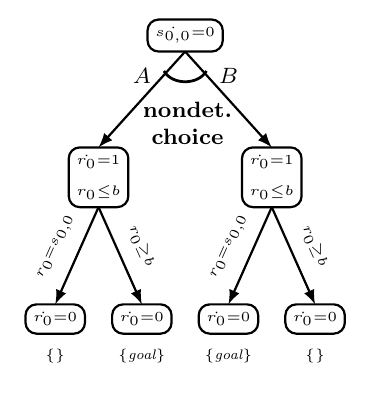
\begin{tikzpicture}[
    %scale=0.1,
    %framed,
    grow=down,
    level 1/.style={sibling distance=2.2cm,level distance=1.8cm},
    level 2/.style={sibling distance=1.1cm, level distance=1.8cm},
    %level 3/.style={sibling distance=1cm, level distance=1.5cm},
    edge from parent/.style={thick,draw=black, ->, >=latex},
    edge from parent path={(\tikzparentnode.south) -- (\tikzchildnode.north)},
    kant/.style={text width=2cm, text centered}, %sloped
    every node/.style={text ragged, inner sep=2mm, outer sep=0cm, font=\footnotesize},
    punkt/.style={inner sep=1mm, rectangle, rounded corners, draw=black, thick, font=\small }
    ]
    \useasboundingbox (-2,0.1) rectangle (2,-4.2);
\node[punkt][rectangle] {$\scriptscriptstyle\dot{s_{0,0}} = 0$}
    child {
        node[punkt, align=center] {$\scriptscriptstyle\dot{r_0} = 1$\\$\scriptscriptstyle r_0\leq b$}
            child {
                node[punkt, label={below:\footnotesize $\scriptscriptstyle\{\}$}] {$\scriptscriptstyle\dot{r_0} = 0$} % no goal
            edge from parent
                node[sloped, kant, above, pos=.5] {\footnotesize $\scriptscriptstyle r_0=s_{0,0}$}
            }
            child {
                node[punkt, label={below:\footnotesize $\scriptscriptstyle\{\textit{goal}\}$}] {$\scriptscriptstyle\dot{r_0} = 0$} % goal
            edge from parent
                node[sloped, kant, above, pos=.5] {\footnotesize $\scriptscriptstyle r_0\geq b$}
            }
        edge from parent
                node[kant, above] {$A$}
    }
    child {
        node[punkt, align=center] {$\scriptscriptstyle\dot{r_0} = 1$\\$\scriptscriptstyle r_0\leq b$}
            child {
                node[punkt, label={below:\footnotesize $\scriptscriptstyle\{\textit{goal}\}$}] {$\scriptscriptstyle\dot{r_0} = 0$} % goal
            edge from parent
                node[sloped, kant, above, pos=.5] {\footnotesize $\scriptscriptstyle r_0=s_{0,0}$}
            }
            child {
                node[punkt, label={below:\footnotesize $\scriptscriptstyle\{\}$}] {$\scriptscriptstyle\dot{r_0} = 0$} % no goal
            edge from parent
                node[sloped, kant, above, pos=.5] {\footnotesize $\scriptscriptstyle r_0\geq b$}
            }
        edge from parent
                node[kant, above] {$B$}
    };


\draw [-,line width=1pt] (0.27,-0.45) to[bend left=60,looseness=1] (-0.27,-0.45) node[below, xshift=0.3cm, yshift=-0.2cm,align=center] {\footnotesize\textbf{nondet.} \\\footnotesize \textbf{choice}};
\end{tikzpicture}
}%
    \only<4>{\begin{tikzpicture}[
    %scale=0.1,
    %framed,
    grow=down,
    level 1/.style={sibling distance=2.5cm,level distance=2cm},
    level 2/.style={sibling distance=1.2cm, level distance=2.2cm},
    %level 3/.style={sibling distance=1cm, level distance=1.5cm},
    edge from parent/.style={thick,draw=black, ->, >=latex},
    edge from parent path={(\tikzparentnode.south) -- (\tikzchildnode.north)},
    kant/.style={text width=2cm, text centered}, %sloped
    every node/.style={text centered, inner sep=2mm, outer sep=0cm, font=},
    punkt/.style={inner sep=0.5mm, rectangle, rounded corners, draw=black, thick, font=\small, text width=1cm }
    ]
    \useasboundingbox (-2,0.1) rectangle (2,-4.2);
\node[punkt][rectangle] {$\dot{r_{0}} = 0$ \\ $\dot{x} = 1$}
    child {
        node[punkt, align=center] {$\dot{r_0} = 1$\\ $\dot{x} = 1$\\\textcolor{orange100}{$ x\leq b$}}
            child {
                node[punkt, label={below: $\{\}$}] {$\dot{r_0} = 0$} % no goal
            edge from parent
                node[sloped, kant, above, pos=.5] { $ r_0$ exp.}
            }
            child {
                node[punkt, label={below: $\{\textit{goal}\}$}] {$\dot{r_0} = 0$} % goal
            edge from parent
                node[sloped, kant, above, pos=.5, orange100] { $ x\geq b$}
            }
        edge from parent
                node[kant, above] {$A$}
    }
    child {
        node[punkt, align=center] {$\dot{r_0} = 1$\\ $\dot{x} = 1$\\\textcolor{orange100}{$ x\leq c$}}
            child {
                node[punkt, label={below: $\{\textit{goal}\}$}] {$\dot{r_0} = 0$} % goal
            edge from parent
                node[sloped, kant, above, pos=.5] { $ r_0$ exp.}
            }
            child {
                node[punkt, label={below: $\{\}$}] {$\dot{r_0} = 0$} % no goal
            edge from parent
                node[sloped, kant, above, pos=.5, orange100] { $ x\geq c$}
            }
        edge from parent
                node[kant, above] {$B$}
    };


\draw [-,line width=1pt] (0.27,-0.6) to[bend left=60,looseness=1] (-0.27,-0.6) node[below, xshift=0.3cm, yshift=-0.2cm,align=center] {\textbf{nondet.} \\ \textbf{choice}};
\end{tikzpicture}
}%
  \end{minipage}%

\end{frame}

%########################################################

\begin{frame}{Case study}
  \begin{minipage}[t]{.6\linewidth}
    \begin{itemize}
      \item Constant inflow
      \item Non-deterministic choice of outflow-valve
      \item Chosen valves stay active for a fixed time
      \item After using a valve, it is blocked for a random amount of time
    \end{itemize}
  \end{minipage}%
  \begin{minipage}[t]{.4\linewidth}
    \centering
    Sketch


    \newcommand{\valve}[1]{\coordinate(A) at #1;% 
\draw[thick] (A) -- ++(0,-1);%
\draw[thick,fill=white] ($(A) + (0,-0.1)$) --++(-0.2,0) --++(0.4,-0.8) --++(-0.4,0) --++(+0.4,0.8) -- cycle;
}
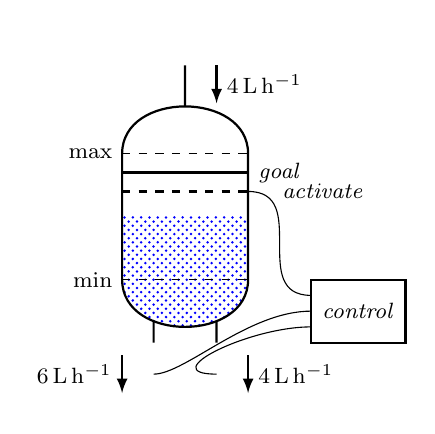
\begin{tikzpicture}
[
    scale=0.8
    ,>=latex
]

    %\draw[help lines] (0,0) grid (7,7);

% tank filling
\begin{scope}
    \clip (0,2) .. controls (0,1) and (2,1) .. (2,2) -- (2,4) .. controls (2,5) and (0,5) .. (0,4) -- cycle;
    
    \fill[pattern=crosshatch dots, pattern color=blue] (0,0) rectangle (4,3);
\end{scope}

% tank body
\draw[thick, name path=tank] (0,2) .. controls (0,1) and (2,1) .. (2,2) -- (2,4) .. controls (2,5) and (0,5) .. (0,4) -- cycle;

% tank labels
\draw[dashed] (0,2) -- node[left,pos=0, font=\footnotesize]{$\min$}(2,2);
\draw[dashed] (0,4) -- node[left,pos=0, font=\footnotesize]{$\max$}(2,4);
\draw[thick] (0,3.7) -- node[right, pos=1, font=\footnotesize]{$\mathit{goal}$} (2,3.7);
\draw[thick, dashed] (0,3.4) -- node[right, pos=1,xshift=0.3cm, font=\footnotesize]{$\mathit{activate}$}(2,3.4);

% controller
\draw[thick] (3,1) rectangle (4.5,2);
\node[font=\footnotesize] at(3.75,1.5) {$\mathit{control}$};

% sensor & wiring
\draw[] (2,3.4) .. controls (3,3.4) and (2,1.75) .. (3,1.75);
\draw[] (0.5,0.5) .. controls (1,0.5) and (2,1.5) .. (3,1.5);
\draw[] (1.5,0.5) .. controls (0.5,0.5) and (2,1.25) .. (3,1.25);

% inflow
\path[name path=outPipeA] (0.5,3) -- (0.5,0);
\path [name intersections={of=tank and outPipeA,by=outNozzleA}];
\path[name path=outPipeB] (1.5,3) -- (1.5,0);
\path [name intersections={of=tank and outPipeB,by=outNozzleB}];
\valve{(0.5,1)}
\valve{(1.5,1)}
\draw[thick] (0.5,1) -- (outNozzleA);
\draw[thick] (1.5,1) -- (outNozzleB);


% outflow
\path[name path=inPipe] (1,6) -- (1,3);
\path [name intersections={of=tank and inPipe,by=inNozzle}];
\draw[thick] (inNozzle) -- (1,5.4);
%\valve{(1,6)}

% labels
\draw[thick,->] (1.5,5.4) --node[right, font=\footnotesize]{\SI{4}{\litre\per\hour}} (1.5,4.8);
\draw[thick,->] (0,.8) --node[left, font=\footnotesize]{\SI{6}{\litre\per\hour}} (0,.2);
\draw[thick,->] (2,.8) --node[right, font=\footnotesize]{\SI{4}{\litre\per\hour}} (2,.2);

\end{tikzpicture}
  \end{minipage}%

\end{frame}

%########################################################

\begin{frame}{Conclusion \& prospect}

\begin{itemize}
  \item Compute optimal probabilities for prophetic and non-prophetic schedulers
  \item No discretization required
  \item Similar complexity for both scheduler types
\end{itemize}

\bigskip

Prospect
\begin{itemize}
  \item Further types of non-determinism
  \begin{itemize}
    \item Non-deterministic rates (e.g., rectangular automata)
    \item Non-deterministic jump times
  \end{itemize}
  \item Other state set representations
\end{itemize}

\end{frame}

%########################################################

\end{document}
